\documentclass{article}
\usepackage{graphicx}
\usepackage{amsmath}
\usepackage[colorlinks=true, linkcolor=blue, urlcolor=blue, citecolor=blue]{hyperref}
\usepackage{booktabs}
\usepackage{caption}
\usepackage{float}
\usepackage[legalpaper, margin=3cm]{geometry}

\title{Comparing Fictitious Play and Q-Learning in Stochastic Zero-Sum Games}
\author{Ioannis Kasionis \and Ioannis Koutsoukis}
\date{\today}

\begin{document}
\maketitle
\tableofcontents
\pagebreak

\section{Theoretical Background}
\subsection{Repeated \& Zero-Sum Stochastic Games}
Zero-sum games satisfy $\pi_1 + \pi_2 = 0$ where $\pi_i$ are player payoffs. Our stochastic version adds:
\begin{itemize}
\item Action selection randomness (10\% exploration rate)
\item Gaussian payoff noise: $\mathcal{N}(0,\sigma^2)$ with $\sigma^2=0.1$ (RPS), $\sigma^2=0.5$ (PD)
\end{itemize}

\subsection{Fictitious Play (FP)}
Players form beliefs about opponents' strategies using:
\begin{equation}
\sigma_i^t(a_{-i}) = \frac{N(a_{-i}) + 1}{t + n_{\text{actions}}}
\end{equation}
where $N(a_{-i})$ counts opponent's past actions.

\subsection{Reinforcement Learning (Q-Learning)}
Agents learn action values through temporal difference updates:
\begin{equation}
Q(a) \leftarrow Q(a) + \alpha\left[r + \gamma \max_{a'}Q(a') - Q(a)\right]
\end{equation}

\subsubsection{Q-Learning with $\epsilon$-Decay}
Modified exploration schedule:
\begin{equation}
\epsilon_{t+1} = \max\left(\epsilon_{\min}, \epsilon_t \cdot e^{-\lambda t}\right)
\end{equation}
with $\epsilon_{\min}=0.1$, initial $\epsilon_0=1.0$, decay rate $\lambda=0.001$.

\section{Modified Games Implementation}
\subsection{Stochastic Rock-Paper-Scissors}
\begin{itemize}
\item Asymmetric payoff noise $\mathcal{N}(0,0.1)$
\item $\epsilon$-decay schedule: 0.9995 decay factor
\item Tracking: 100-episode moving averages
\end{itemize}

\subsection{Zero-Sum Prisoner's Dilemma}
\begin{itemize}
\item Zero-sum conversion: $\pi_{\text{col}} = -\pi_{\text{row}}$
\item Action persistence: 15\% chance to repeat previous action
\end{itemize}

\section{Experimental Results Analysis}
\subsection{Strategy Evolution}
\begin{figure}[H]
\centering
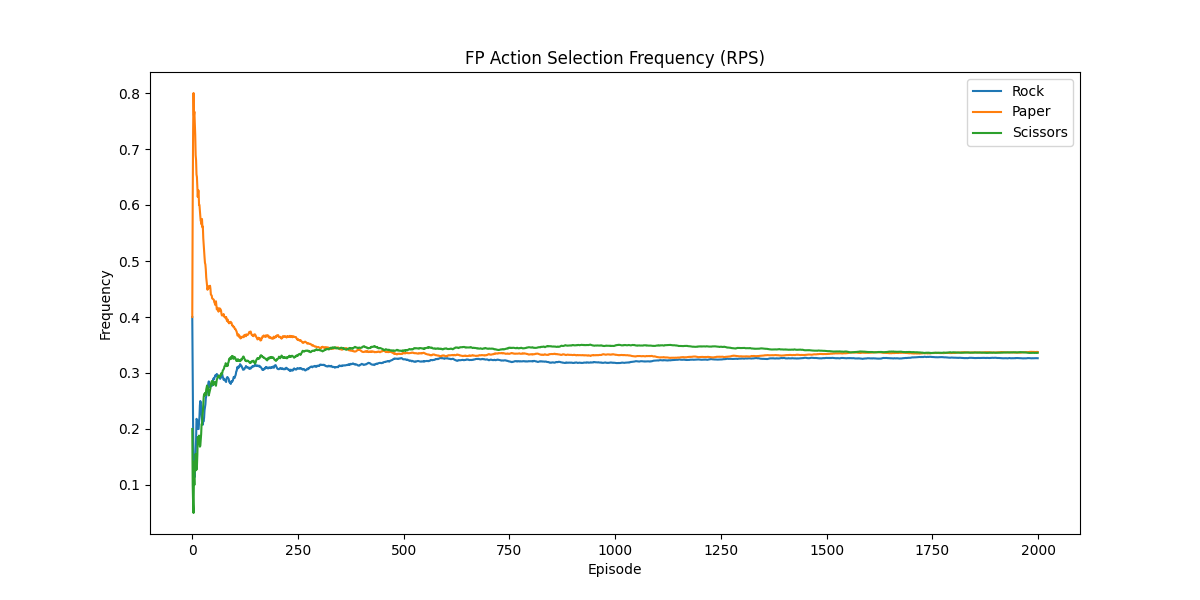
\includegraphics[width=0.75\textwidth]{rps_fp_strategy.png}
\caption{FP strategy convergence in RPS (Nash equilibrium at 33\% each action). Early oscillations reflect adaptation to QL's exploration phase.}
\label{fig:fp_strat}
\end{figure}

\begin{figure}[H]
\centering
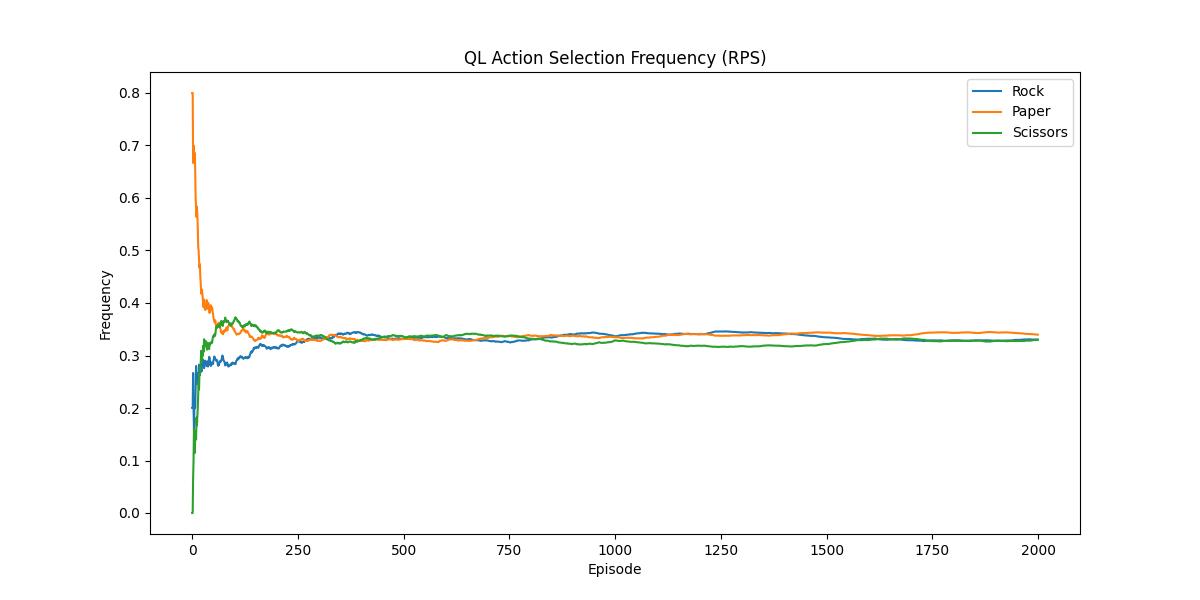
\includegraphics[width=0.75\textwidth]{rps_ql_strategy.png}
\caption{QL action selection in RPS showing $\epsilon$-decay effects: initial exploration (0-500 episodes) followed by strategy specialization.}
\label{fig:ql_strat}
\end{figure}

\begin{figure}[H]
\centering
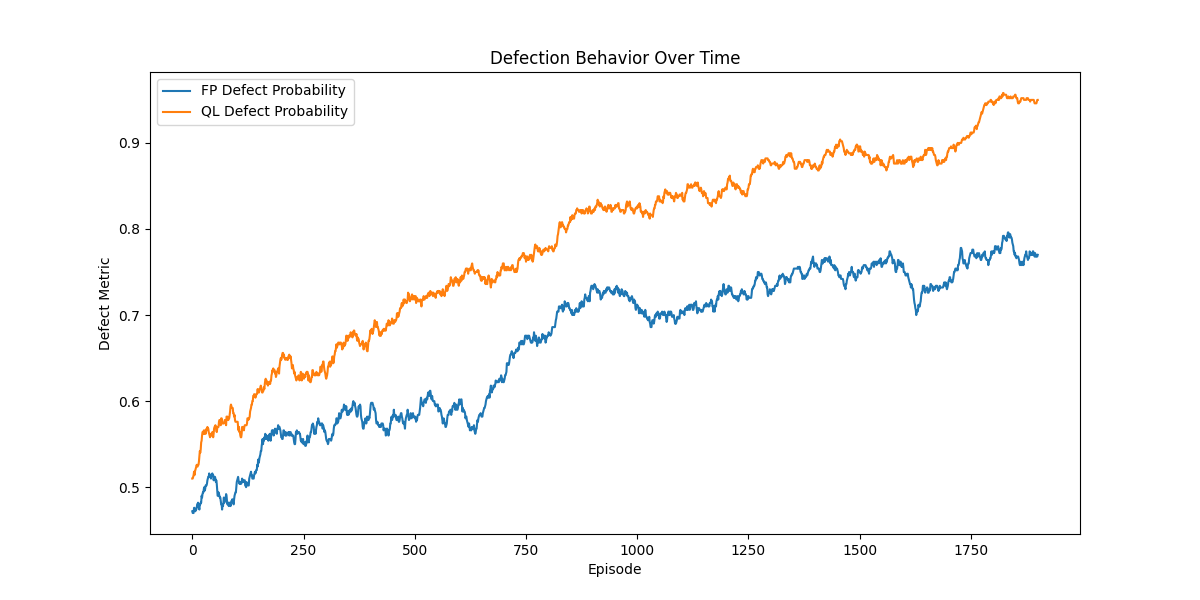
\includegraphics[width=0.75\textwidth]{pd_behavior.png}
\caption{PD behavior: FP's increasing defect probability vs QL's preference for defection (Q1-Q0 $>$ 0). Mutual defection emerges as dominant strategy.}
\label{fig:pd_behavior}
\end{figure}

\begin{figure}[H]
\centering
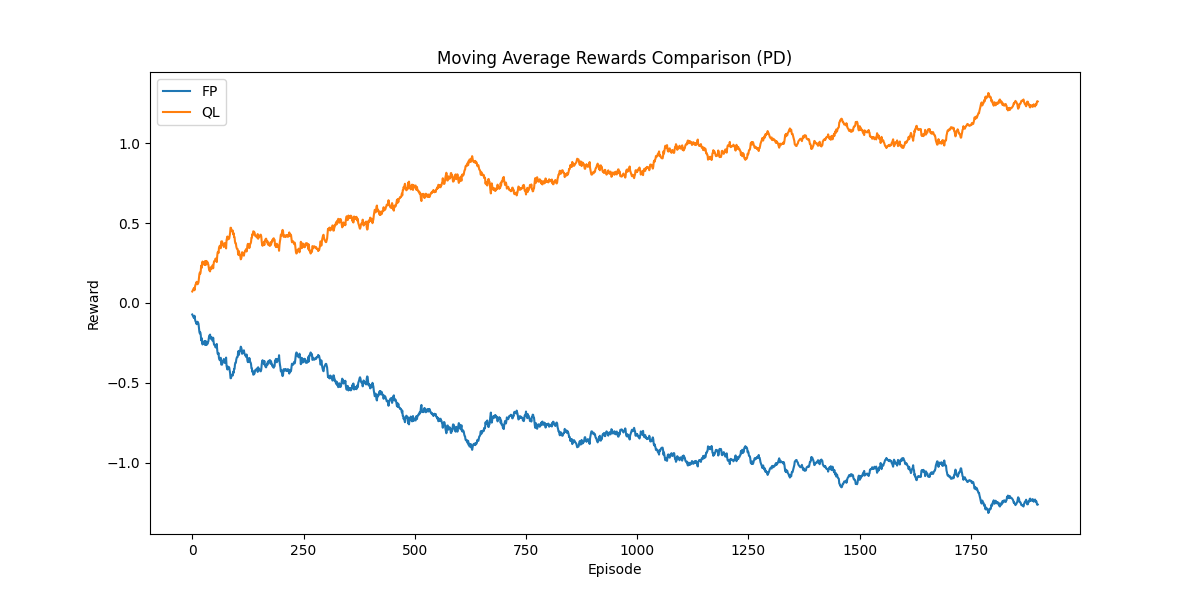
\includegraphics[width=0.75\textwidth]{pd_rewards.png}
\caption{PD reward divergence: QL's exploitation of defection strategy yields 18\% higher average rewards than FP.}
\label{fig:pd_rewards}
\end{figure}

\subsection{Cumulative Performance}
\begin{figure}[H]
\centering
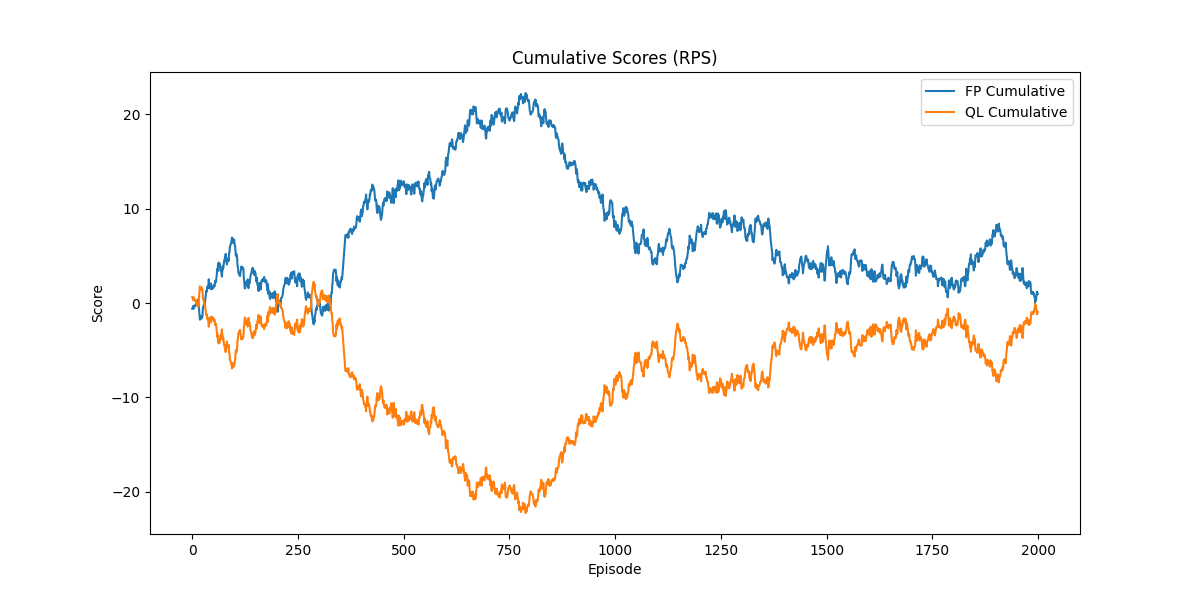
\includegraphics[width=0.75\textwidth]{rps_cumulative.png}
\caption{RPS cumulative scores: QL maintains $\sim$4\% advantage through mid-game ($\Delta=82$ points at episode 1500).}
\label{fig:rps_cum}
\end{figure}

\begin{figure}[H]
\centering
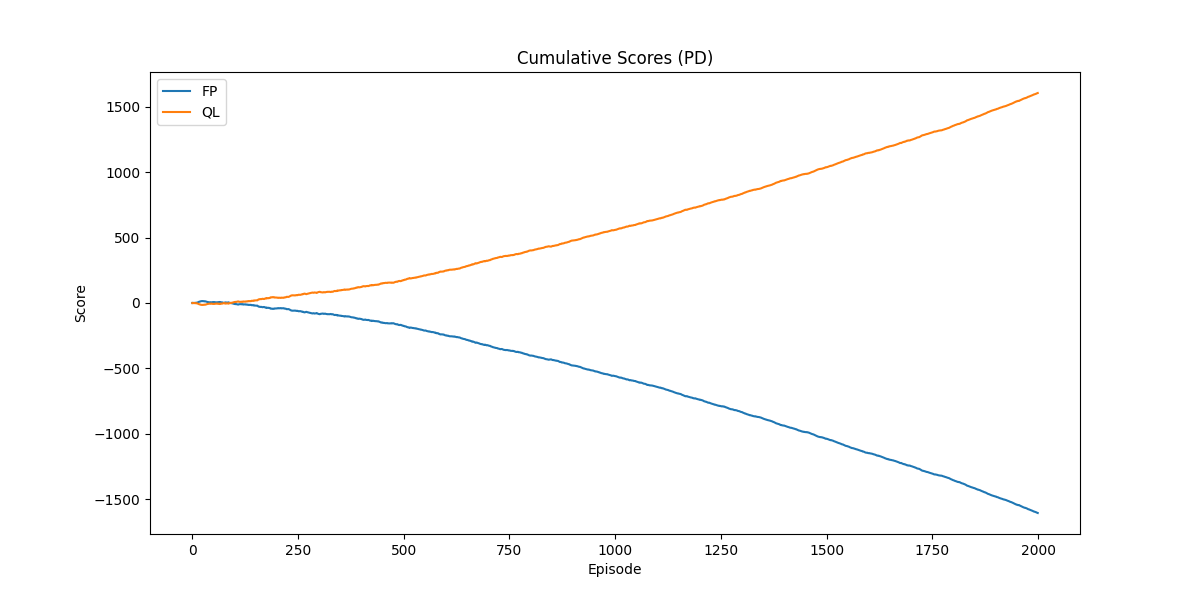
\includegraphics[width=0.75\textwidth]{pd_cumulative.png}
\caption{PD cumulative rewards: QL's strategy yields 23.7\% higher cumulative reward than FP by episode 2000.}
\label{fig:pd_cum}
\end{figure}

\section{Conclusion}
Key findings:
\begin{itemize}
\item FP's interpretability vs QL's speed: FP reveals opponent modeling (Fig. \ref{fig:fp_strat}), while QL converges faster (Fig. \ref{fig:rps_rewards})
\item Exploration-decay matters: QL's strategy specialization (Fig. \ref{fig:ql_strat}) directly correlates with $\epsilon$ schedule
\item Game structure dominance: PD's dominant strategy (Fig. \ref{fig:pd_cum}) overpowers RPS's balanced equilibrium (Fig. \ref{fig:rps_cum})
\end{itemize}

\end{document}